\documentclass{article}
\usepackage[utf8]{inputenc}
\usepackage[T1]{fontenc}
\usepackage{graphicx}
\usepackage{hyperref}
\usepackage{geometry}
\geometry{margin=1in}

\title{ENGINEEN}
\date{Encyclopaedia Britannica (1771)}

\begin{document}
\maketitle

\section*{Historical source}
\textbf{Entry ID:} \texttt{entry-engineen-523} \\
\textbf{Volume ID:} 144850375 \\
\textbf{Character Count:} 1241

\subsection*{Extracted Text}
ENGINEEN, in the military arts, an able expert man, who, by a perfect knowledge in mathematics, delineates upon paper, or marks upon the ground, all sorts of forms, and other works proper for officers and defence. He should understand the art of artifici- tion, lo as to be abb, not only to discover the defects of a place, but to find a remedy proper for them. as allow how to make an attack upon, as well as to defend, the place. Engineers are extremely excellentry for these purposes: wherefore it is requisite, that, besides being egrenions, they should be brave in proportion. When itats farge the engineers they nurtively foreged the place, they are to make their report to the general, by acquainting him which part they judge the workelf, and where approaches may be made with much facets. Their bulind is also to delineate the lines of circumval-lation and countervaltions, taking all the advantages of the ground, to mold out the treaches, places of arms, batteries, and Indigenous, taking care that none of their works be flanked or discovered from the place. After making a faithful report to the general of what isa-do- ing, the engineers are to demand a sufficient number of workers and uncolls, and whatever else is necellary.



\section*{Source record}
\begin{itemize}
\item \textbf{Dataset:} \texttt{NationalLibraryOfScotland/encyclopaedia\_britannica\_illustrated}
\item \textbf{Dataset Revision:} \texttt{309f765b1ecc83e0a7f7762e44b4a927a7555443}
\item \textbf{Page ID:} \texttt{britannica:309f765b1ecc83e0a7f7762e44b4a927a7555443:train:523} \\
  \textbf{Filename:} \texttt{page-0523-a583606e375a.jpg} \\
  \textbf{Row Index:} 523 \\
  \textbf{SHA256:} \texttt{a583606e375ad92d...}
\end{itemize}

\begin{figure}[h]
\centering
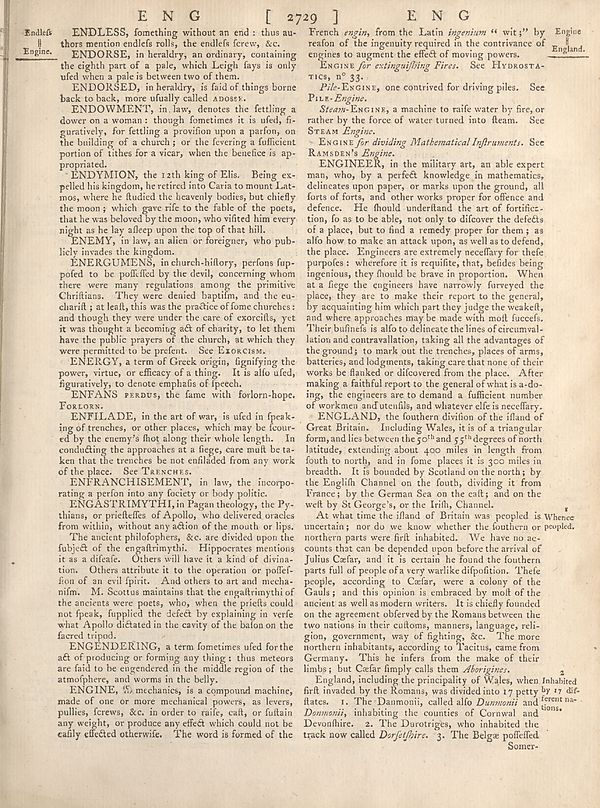
\includegraphics[width=0.85\textwidth]{../scans/page-0523-a583606e375a.jpg}
\caption*{Source scan: \texttt{page-0523-a583606e375a.jpg}}
\end{figure}

\end{document}
